\subsection{Dokumentation}
\subsubsection{Dokumentation des ML-Algorithmus}
Für die Dokumentation des Algorithmus kann sich an Model Cards for Model Reporting orientiert werden.
\todo[inline]{Hier erkläre ich noch Model Cards for Model Reporting}
Es existieren auch Beispiele für die Anwendung von Model Cards for Model Reporting in der medizinischen Branche \cite{sendak2020human} sowie der Biologie \cite{grasso2020applying}.

Daneben können zur Dokumentation des Algorithmus auch Grafiken genutzt werden, welche häufig schon während der Entwicklung angewendet werden. So könnte eine Confusion-Matrix \cite{hasib2022machine} genau so wie die Darstellung von Precision, Recall, Specificity und F1-Score \cite{huvc2021anomaly} mit in die Dokumentation einfließen.
\todo[inline]{Hier werde ich noch kurz erklären, was die Metriken aussagen und vlt. Bilder einbauen}

\subsubsection{Dokumentation der Modellauswahl}
Auch die Modellauswahl sollte dokumentiert werden. So kann von Interesse sein, welche Verfahren ausprobiert wurden. Weiter könnte dokumentiert werden, ob oder wann z.B. um Überanpassung zu vermeiden mit dem Training gestoppt wurde \cite{de2018algorithmic}.

\subsubsection{Ganzheitliche Dokumentation}
Ein bekanntes Beispiel für die ganzheitliche Dokumentation eines ML-Systems ist ABOUT ML. Dies ist eine Sammlung von Best Pratices zur Dokumentation von Daten, Modellen und betrachtet hierbei den gesamten Lebenszyklus \cite{vaughan2020human, raji2019ml}. Daneben werden auch Artefakte oder Prozesse dokumentiert und es richtet sich an unterschiedliche Arten von Stakeholdern \cite{raji2019ml}.

Ein Framework, an dem sich bei der Dokumentation orientiert werden kann, wurde von \cite{hernandez2021explainable} im Bereich der Luftfahrt entwickelt. Dieses sollte zwar ursprünglich  setzt zwar den initialen Fokus darauf Vertrauen zu schaffen, aber kann auch zu mehr Transparenz beitragen. Aspekte, welche in die Dokumentation mit einfließen könnten, sind:
\begin{itemize}
    \item Zweck des Systems: Was macht der Algorithmus? Welcher Algorithmus wurde aus welchen Gründen ausgewählt (mögliche Gründe: Performance oder Genauigkeit)?
    \item Technische Robustheit: Datenquellen (Qualität, Zugang, Integrität, Schutz und Sicherheit), Lebenszyklus, Zuverlässigkeit, Reproduzierbarkeit, Interpretierbarkeit/Erklärbarkeit
    \item Maßnahmen im Bereich der IT-Sicherheit
    \item Darstellung von nutzerfreundlichen Erklärungen sowie Reporting und Auditing
\end{itemize}

Ein weiteres Framework wurde von \cite{garbin2022assessing} entwickelt. Dieses legt zwar auch den Fokus eher auf Audits von ML-Systemen, kann jedoch auch dabei helfen ein System transparenter zu machen. In folgender Aufzählung sind kurz die wichtigsten Aspekte dargestellt, gekürzt um die Punkte, welche sich konkret auf das Durchführen von Audits beziehen:
\todo[inline]{Die beiden Checklisten gieße ich eventuell noch in den Text - auf jeden Fall fließen die Inhalte irgendwie in meine Handreichung ein, da besonders die zweite Abbildung meine dritte Forschungsfrage beantwortet}
\begin{itemize}
    \item Scoping: Dokumentation der Systemanforderungen und der angewendeten ML-Prinzipen, Use-Cases für ein ethisches Review und einer social impact analysis
    \item Mapping: Mapping von Stakeholdern auf Anforderungen, Dokumentation der Stakeholder-Interviews
    \item Artefakte: Checklisten, Model Cards, Datasheets for Datesets
    \item Testen: gegenseitige Prüfung der Dokumentation
    \item Reflektion: Zeitplan
\end{itemize}
Zusätzlich geben \cite{garbin2022assessing} einen Überblick über mögliche Checklisten und geben an, welche Checkliste in welchem zeitlichen Stadium der ML-Entwicklung \ref{Fig:ChecklisteJeStadium} angewendet wird und an wen diese sich richtet \ref{Fig:ChecklisteJeRolle}.
\begin{figure}[h]
    \centering
    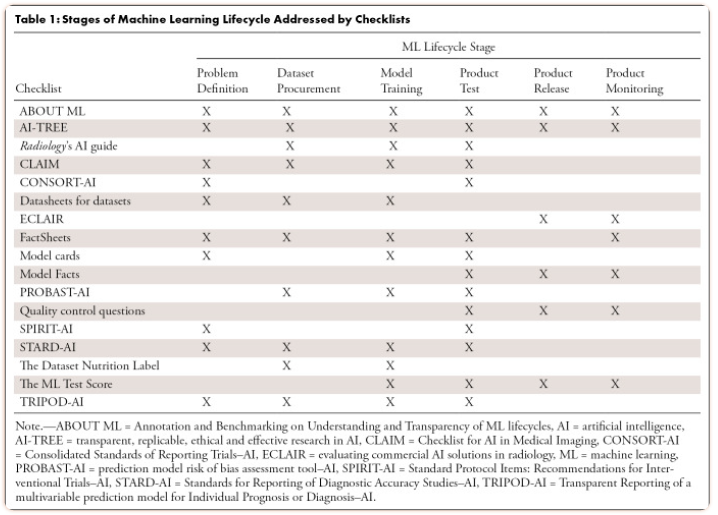
\includegraphics[scale=0.45]{pic/MA-Bilder/Literaturrecherche/49-ChecklistNachStages.PNG}
    \caption{Checkliste je ML-Stadium, entommen aus: \cite{garbin2022assessing}}
    \label{Fig:ChecklisteJeStadium}
\end{figure}
\begin{figure}[h]
    \centering
    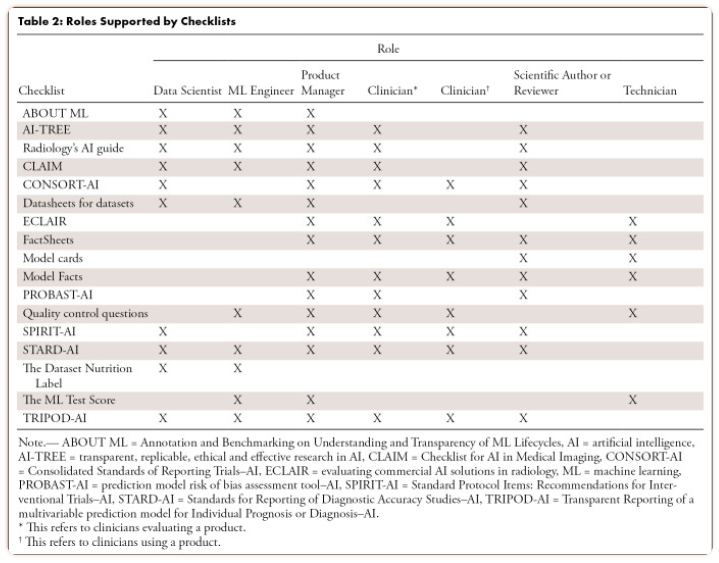
\includegraphics[scale=0.45]{pic/MA-Bilder/Literaturrecherche/49-ChecklistNachRollen.PNG}
    \caption{Checkliste je Publikum, entommen aus: \cite{garbin2022assessing}}
    \label{Fig:ChecklisteJeRolle}
\end{figure}

Weiterführend finden sich in der Veröffentlichung von \cite{garbin2022assessing} Hinweise darüber, wann welche Dokumentationsmethode eingesetzt werden kann. Konkret gehen sie auf Datasheets for Datasets, Modelcards und Modelfact ein (siehe Abbildung \ref{Fig:Datsheet_Datest_Modelfact}).
\begin{figure}
    \centering
    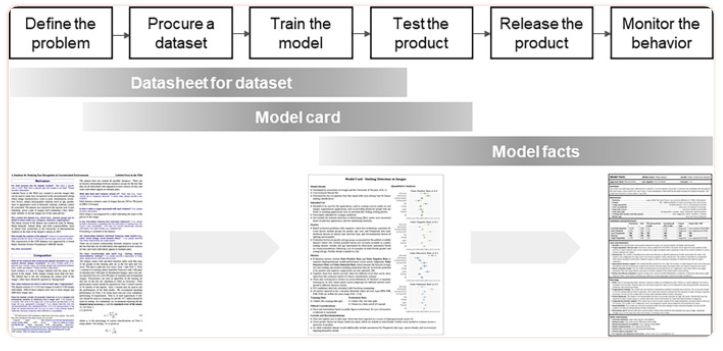
\includegraphics[scale=0.45]{pic/MA-Bilder/Literaturrecherche/49-ZusammenspielDatasheets_Modelcard_Modelfacts.PNG}
    \caption{Übersicht XAI-Methode mit Audience, entommen aus: \cite{garbin2022assessing}}
    \label{Fig:Datsheet_Datest_Modelfact}
\end{figure}